\section{Verbundgenerator}
Die letzte zu untersuchende Maschine ist ein Verbundgleichstromgenerator. Dieser vereint in unserem Fall einen fremderregten Generator mit einem Reihenschlussgenerator. Dazu wird die Fremderregerwicklung sowie die Reihenschlusswicklung wie in Abbildung \ref{abb:verbund_BKL_Messschaltung} verschaltet. Dadurch wird das Hauptfeld in Abhängigkeit von $R_S$ proportional zum Ankerstrom erhöht, wodurch zum Beispiel die Ankerrückwirkung reduziert werden kann. Die Erregung ist nun über zwei Widerstände regelbar - einerseits über den Fremderregerwiderstand, andererseits durch Variation des zur Hilfsreihenschlusswicklung parallel geschalteten Widerstands $R_S$. Wird dieser erhöht, fließt mehr Ankerstrom durch die Wicklung, was eine erhöhte Erregung zur Folge hat. Bei Verringerung des Widerstandes zapft dieser in der Parallelschaltung mehr Strom ab, wodurch die Erregerdurchflutung sinkt. 

\begin{figure} [htb]
    \centering
    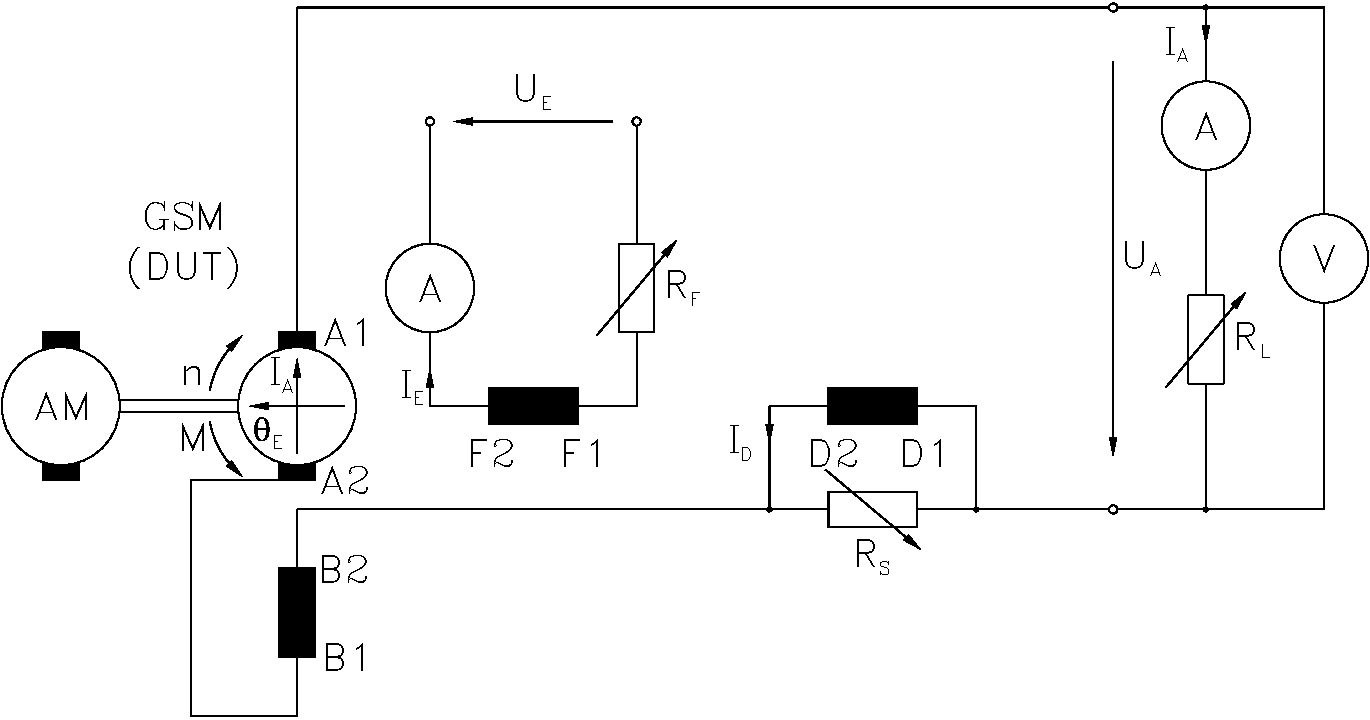
\includegraphics[width=0.75\textwidth, angle=0]{\currfiledir images/Belastungskennlinie_verbunderregt}
    \caption{Messschaltung zur Ermittlung der äußeren Kennlinie des Verbund\-gleich\-strom\-generators (GSM) - Reihenschlusswicklung hier dargestellt für Kompoundierung (für Gegenkompoundierung müssen die Anschlüsse der Reihenwicklung $D1$ und $D2$ vertauscht werden).}
    \label{abb:verbund_BKL_Messschaltung}
\end{figure}

\subsection{Äußere Kennlinie}

Bei der äußeren Kennlinie wurden drei verschiedene Konfigurationen - überkompoundiert, kompoundiert und gegenkompoundiert - aufgenommen, auf die in Folge näher eingegangen wird. Dabei wurde jeweils der Widerstand $R_S$ fix vorgegeben und der Belastungswiderstand $R_L$ bei Nenndrehzahl und Nenn-Fremderregung ($I_{F,N}= \SI{1.75}{\ampere}$) variiert. Abbildung \ref{abb:verbund_kennlinien} zeigt die gemessenen äußeren Kennlinien als durchgezogene Linien für jeden dieser Fälle.

\subsubsection{Überkompoundiert}

Bei der Überkompoundierung ist es nicht nur das Ziel, die Ankerrückwirkung zu kompensieren, sondern darüber hinaus die Erregung proportional mit dem Ankerstrom zu verstärken und damit im Generatorbetrieb eine erhöhte Ankerspannung zu erhalten. Die abnehmende Steigung der Kennlinie bei zunehmendem Strom rührt aus der maximal verfügbaren Leistung der Antriebsmaschine. 

\subsubsection{Kompoundiert}

Bei der reinen Kompoundierung wird versucht, das schwächende Feld der Ankerrückwirkung durch die Hilfsreihenschlusswicklung exakt zu kompensieren und somit eine belastungsunabhängige Charakteristik zu erzielen. Es ist zu erkennen, dass dies nicht gänzlich gelingt - für ein noch besseres Ergebnis wäre der Parallelwiderstand $R_S$ weiter zu senken. 

\subsubsection{Gegenkompoundiert}

Vertauscht man die Klemmen der Hilfsreihenschlusswicklung, so wird der gegenteilige Effekt erzielt: Das von ihr erzeugte Feld wirkt zusammen mit der Ankerrückwirkung der Erregung entgegen und bewirkt damit ein starkes Einbrechen der Ankerspannung mit steigendem Strom.

\subsection{Innere Kennlinien}

Für die inneren Kennlinien der verschiedenen Betriebszustände werden die äußeren herangezogen und entsprechend 

\begin{equation}
U_i=U_A+I_A R_A
\end{equation}

\noindent umgerechnet. Der vergleichsweise ohnehin niedrige Widerstand der Hilfsreihenschlusswicklung $R_D$ wird durch die Paralllelschaltung mit $R_S$ weiter verringert, weshalb diese vernachlässigt und nur der Ankerkreiswiderstand herangezogen wird. Die Ergebnisse sind ebenfalls in Abbildung \ref{abb:verbund_kennlinien} grafisch dargestellt, im Gegensatz zu den äußeren Kennlinien jedoch strichliert.

\input{\currfiledir Verbund}
%\input{\currfiledir schaltung}